\section{管理属性}
\footnote{{\bf 重要:}如果你用过老版本的~Cytoscape就会发现属性的处理方式已经发生了
改编。其中,最重要的变化是属性不再是存放在当前目录或主目录的.cytoscape目录中,而是
保存在Cytoscape的会话文件中(后缀是.cys)。在.cytoscape目录下肯定会有一个
cytoscape.props文件,但这个文件只有当用户要求将但前属性保存为缺省属性时才会被修改。
除非实在是有什么特别的原因,否则还是用缺省设置比较好。}

用菜单上的Edit → Preferences → Properties…可以打开Cytoscape的属性编辑器,在这里可以
修改各种属性。对于一般的属性,都是保存在Cytoscape的会话文件中,所以只对当前会话有效。
只有将其设为缺省属性,或是用File → Export将其导出,才能在其他的会话中生效。

可以通过~Add~(添加)、Modify~(修改)和~Delete(删除)操作来配置~Cytoscape~的属性。\\
\begin{center}
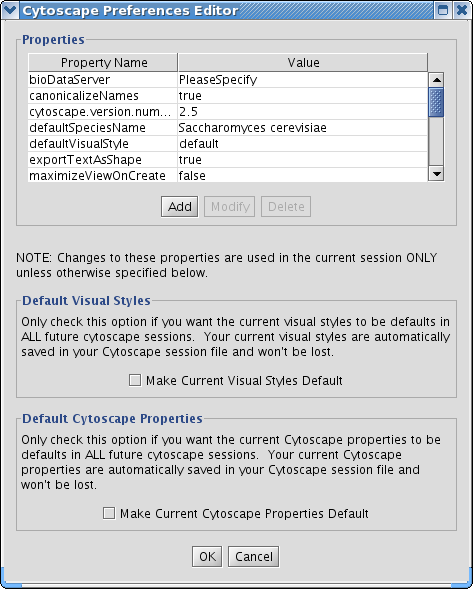
\includegraphics[width=\textwidth]{images/prefs_editor.png} 
\end{center}

 下面介绍一些常见的属性。
\begin{table}[!h]
\begin{tabular}{|c|c|p{5.5cm}|}
\hline 
 \textbf{属性名称}& \textbf{缺省值}& \textbf{有效值}\\ \hline
 viewThreshold& 10000&大于0的整数\\ \hline
 secondaryViewThreshold& 30000& 大于0的整数 \\ \hline
 viewType& tabbed& tabbed \\ \hline
 defaultWebBrowser & &
 指向系统默认浏览的路径。只有当~Cytoscape~找不到系统的浏览器时才需要设置这个属性。\\
 \hline 
\end{tabular}
\end{table}

\subsection{设置属性的缺省值}
Cytoscape~的缺省属性是可以修改的。

在~Edit$\rightarrow$Preferences$\rightarrow$Properties\ldots中编辑属性,选上~Make Current Cytoscape Properties Default~。这样,当前属性就会保存到.cytoscape目录中,对每个Cytoscape会话都会生效。否则,这些属性就只会保存到当前会话的.cys文件中,新的会话依然会使用缺省属性。

